\newpage
\section{Fundamentação teórica}\label{chap:fundamentacao-final}

\subsection{Agricultura digital e informações georreferenciadas}

A agricultura digital envolve o uso de dados e sistemas computacionais em atividades agrícolas. Uma área de cultivo não precisa apresentar as mesmas condições em todos os seus pontos, nem manter essas condições ao longo do tempo. Na agricultura de precisão, essas diferenças espaciais e temporais são relevantes para o acompanhamento da área. Revisões sobre aplicações agrícolas de sensoriamento remoto e computação mostram o uso de diferentes sensores, algoritmos e tarefas \citep{WEISS2020,PATRICIO2018}. Neste trabalho, a plataforma disponibiliza informações para consulta e exploração; não realiza prescrição de insumos, controle de máquinas ou recomendação de manejo.

Para analisar uma área, o sistema precisa representar tanto seus limites quanto os valores observados dentro dela. Os limites são descritos por um polígono, no modelo vetorial. Já os valores dos índices são organizados em células de uma grade, no modelo raster \citep{QGIS_VECTOR,QGIS_RASTER}. Como essas informações estão associadas a posições geográficas, podem ser apresentadas juntas no mapa.

No mapa temático, as cores representam os valores conforme a relação indicada na legenda \citep{QGIS_MAP}. Por isso, uma mesma cor não significa necessariamente o mesmo valor em mapas com escalas diferentes. Uma visualização pode ajustar suas cores ao intervalo encontrado na área, enquanto outra mantém um intervalo fixo. A comparação precisa considerar essa diferença, e não apenas a aparência das cores.

\subsection{Sensoriamento remoto multiespectral e Sentinel-2}

Sensores ópticos multiespectrais registram a resposta da superfície em diferentes faixas do espectro eletromagnético, chamadas bandas. Comparar essas bandas permite construir indicadores associados à vegetação e à água. A interpretação depende, porém, do alvo observado, da atmosfera, da geometria de observação e da qualidade dos dados \citep{WEISS2020}.

Na missão Sentinel-2, o instrumento MSI (\textit{MultiSpectral Instrument}) observa treze bandas, com resoluções espaciais nominais de 10, 20 e 60 m. A revisita nominal da configuração de dois satélites é de cinco dias \citep{ESA_SENTINEL2}. Isso não significa que haverá um valor utilizável a cada cinco dias: nuvens, cobertura e filtros podem impedir o aproveitamento de uma aquisição, isto é, de uma imagem obtida pelo sensor.

O sistema utiliza a coleção \texttt{COPERNICUS/S2\_SR\_HARMONIZED}, que fornece produtos Level-2A de reflectância de superfície. Esses dados já passaram pelo processamento do produto; a aplicação não realiza calibração do instrumento ou correção atmosférica própria. A coleção harmonizada também ajusta diferenças introduzidas por mudanças na linha de processamento. O produto catalogado contém doze bandas espectrais, sem B10, além de bandas auxiliares de qualidade. Seus valores de reflectância são fornecidos com fator de escala $10^{-4}$ \citep{GOOGLE_S2_SR}.

As bandas usadas nos índices não observam exatamente as mesmas faixas nem possuem todas a mesma resolução. B4 registra o vermelho e B8 o infravermelho próximo (NIR, \textit{Near Infrared}) amplo, ambas com resolução nominal de 10 m. B8A registra uma faixa mais estreita do NIR, enquanto B11 registra o infravermelho de ondas curtas (SWIR, \textit{Shortwave Infrared}); as duas têm resolução de 20 m \citep{GOOGLE_S2_SR}.

Ao combinar essas bandas, é necessário distinguir a resolução original da grade escolhida para apresentar ou processar os dados. Solicitar uma grade a 10 m não cria novas observações físicas nas bandas de 20 m. Na reprojeção, o Earth Engine usa vizinho mais próximo por padrão, enquanto outros métodos precisam ser solicitados explicitamente \citep{GOOGLE_EE_RESAMPLE}. A aplicação não solicita interpolação bilinear ou bicúbica.

\subsection{Índices espectrais e nomenclatura}\label{sec:indices-final}

Os três índices implementados comparam duas bandas por uma diferença normalizada: subtraem uma resposta da outra e dividem o resultado pela soma das duas. Para respostas $A$ e $B$, a expressão é $(A-B)/(A+B)$, desde que o denominador não seja nulo. Se as entradas forem não negativas, o resultado fica em $[-1,1]$. Além disso, multiplicar ambas pelo mesmo fator de escala não altera a razão, porque esse fator aparece no numerador e no denominador e se cancela.

Nas expressões, $p$ identifica a posição espacial e $t$ a aquisição. Os símbolos das bandas representam os valores de reflectância escalados do produto.

Essas propriedades não eliminam os cuidados com os dados de entrada. Denominadores nulos, valores inválidos, posições excluídas por máscaras de qualidade e diferenças de resolução precisam ser considerados. A função utilizada no Earth Engine também mascara o pixel, excluindo-o do resultado válido, quando qualquer uma das bandas possui entrada negativa \citep{GOOGLE_EE_ND}.

\subsubsection{NDVI}

O índice de vegetação por diferença normalizada (NDVI, \textit{Normalized Difference Vegetation Index}) relaciona a resposta no NIR à resposta no vermelho, explorando o contraste espectral associado à vegetação. No trabalho de \citet{ROUSE1974_NTRS}, a seção de análise espectral descreve a diferença entre bandas 5 e 7 do ERTS-1 (\textit{Earth Resources Technology Satellite}) dividida por sua soma, denominada \textit{Band Ratio Parameter}, além de uma transformação posterior. Essa base histórica não empregava bandas Sentinel-2. Na implementação deste sistema, B8 representa o NIR e B4 o vermelho:
\begin{equation}\label{eq:ndvi-final}
 NDVI(p,t)=\frac{B8(p,t)-B4(p,t)}{B8(p,t)+B4(p,t)}.
\end{equation}
O NDVI resume o contraste entre as bandas, não uma medida direta de produtividade, biomassa ou sanidade. Em coberturas densas, pode apresentar saturação, reduzindo sua capacidade de distinguir variações; a resposta do solo também pode influenciar o índice \citep{GAO1996}. Condições atmosféricas, geometria de aquisição e estágio da cultura afetam as relações com variáveis agrícolas \citep{WEISS2020}. Quando um pixel contém mais de um tipo de alvo, seu valor não separa a resposta de cada componente. Por essas razões, o sistema não adota faixas universais de classificação agronômica.

\subsubsection{NDWI utilizado na aplicação}

O acrônimo NDWI (\textit{Normalized Difference Water Index}) designa formulações que precisam ser distinguidas pelas bandas utilizadas. \citet{GAO1996} apresentou um índice relacionado à água líquida na vegetação, com bandas próximas de 0,86 e 1,24 µm. B11 do Sentinel-2 situa-se aproximadamente em 1,61 µm \citep{GOOGLE_S2_SR}; portanto, não reproduz a segunda faixa original. Nesta aplicação, o rótulo NDWI identifica a seguinte variante NIR--SWIR:
\begin{equation}\label{eq:ndwi-final}
 NDWI_{\mathrm{sistema}}(p,t)=
 \frac{B8(p,t)-B11(p,t)}{B8(p,t)+B11(p,t)}.
\end{equation}
Essa expressão difere do NDWI verde--NIR destinado à delimitação de água superficial \citep{MCFEETERS1996}. A combinação B8/B11 também aparece sob o nome NDMI na Tabela 1 de \citet{IZQUIERDO2026}. Portanto, a identificação das bandas é necessária para interpretar o indicador, independentemente do acrônimo adotado.

\subsubsection{NDMI utilizado na aplicação}

O Serviço Geológico dos Estados Unidos (USGS) descreve o índice de umidade por diferença normalizada (NDMI, \textit{Normalized Difference Moisture Index}) pela combinação NIR--SWIR em produtos Landsat \citep{USGS_NDMI}. Nesta plataforma, a expressão utiliza B8A, em vez de B8:
\begin{equation}\label{eq:ndmi-final}
 NDMI_{\mathrm{sistema}}(p,t)=
 \frac{B8A(p,t)-B11(p,t)}{B8A(p,t)+B11(p,t)}.
\end{equation}
Na prática, a diferença entre os indicadores chamados NDWI e NDMI nesta aplicação está na banda NIR: o primeiro usa B8 e o segundo B8A, ambos combinados com B11. Como B8 e B8A diferem em faixa espectral e resolução original, os valores podem ser diferentes. Isso não os torna duas medições independentes da umidade do solo.

A combinação B8A/B11 está presente no exemplo executável de NDMI da Sentinel Hub, cuja descrição textual emprega B8/B11 \citep{SENTINELHUB_NDMI}. A disponibilização das duas variantes amplia as possibilidades de exploração espectral, mantendo os identificadores da interface e explicitando suas bandas. Não se estabelece superioridade entre elas.

\subsection{Processamento geoespacial remoto e serviços de referência}

O Earth Engine disponibiliza infraestrutura remota para análise geoespacial \citep{GORELICK2017}, utilizada em diversas aplicações de sensoriamento remoto \citep{AMANI2020}. A aplicação consulta e combina imagens por uma interface de programação de aplicações (API) Python, sem armazenar todo o acervo localmente. Os objetos da API descrevem operações remotas; chamadas como \texttt{getInfo()} transferem resultados ao processo Python. A organização das consultas e o volume transferido são, portanto, decisões relevantes para a interação.

Google Earth, Google Earth Engine, serviço de geocodificação e mapa-base cumprem funções distintas. O software deste trabalho não integra o aplicativo Google Earth. O Earth Engine processa as imagens analíticas; o Nominatim resolve nomes de lugares em coordenadas; o Esri World Imagery fornece a base cartográfica. A aparência fotográfica do mapa-base não identifica a data ou o sensor da imagem usada no cálculo espectral.

\subsection{Agregação espacial e temporal}

Para representar um período em um mapa, o sistema calcula a mediana dos valores válidos do índice em cada posição. Na sequência ordenada, ela corresponde ao valor central para quantidade ímpar e à média dos dois centrais para quantidade par. Sua menor sensibilidade à magnitude dos extremos \citep{NIST_LOCATION} pode atenuar contaminações residuais, sem substituir as máscaras de qualidade. A operação é aplicada por pixel e banda \citep{GOOGLE_EE_MEDIAN}; a composição resultante pode reunir diferentes quantidades de observações e não corresponde necessariamente a uma aquisição.

Outra operação consiste em resumir os valores encontrados dentro da área selecionada, processo chamado redução espacial. Se a média for calculada separadamente para cada imagem, o resultado será uma sequência de médias da área nas datas disponíveis. Se for calculada sobre o mapa composto, o resultado será um único valor que resume esse mapa. A ordem das operações importa: a média espacial das medianas temporais não é, em geral, igual à média ou à mediana das médias por aquisição. As máscaras e os pesos usados na operação também influenciam quais valores contribuem para o resultado \citep{GOOGLE_EE_REDUCE}.

\subsection{Séries temporais, tendência e comportamentos atípicos}

Uma série temporal associa valores a instantes de observação. Quando as imagens são filtradas, os intervalos podem ser irregulares e uma mesma data pode conter mais de um registro. Isso afeta a interpretação dos métodos: uma janela de três observações não tem duração fixa, e uma reta ajustada à posição sequencial dos registros não fornece uma taxa de variação diária. Essas distinções orientam a leitura da tendência e dos desvios apresentados no sistema.

Uma média móvel resume um grupo de observações que se desloca ao longo da série. Já o ajuste de uma reta permite resumir sua direção geral. No método dos mínimos quadrados, a reta é escolhida para minimizar a soma dos quadrados das diferenças entre os valores observados e os valores ajustados \citep{HYNDMAN2021}.

Para examinar um desvio, também é possível comparar sua distância em relação a uma média com a dispersão dos valores de referência, expressa pelo desvio padrão. O resultado dessa padronização é um escore Z. O NIST alerta para suas limitações em pequenas amostras e distingue a sinalização exploratória dos testes formais de valores atípicos \citep{NIST_OUTLIERS}. Nesta aplicação, a referência são observações anteriores, não a média e o desvio amostrais de toda a série. A regra procura apenas quedas relativas: é uma heurística unilateral, não um teste de significância ou um modelo treinado. A ausência de sinalização não comprova condição agronômica normal.

\citet{MERONI2019} empregam escores de NDVI com referência histórica sazonal e examinam um limiar negativo de um desvio padrão. O estudo utiliza dados MODIS e procedimentos de suavização e consolidação. Essa aplicação oferece um precedente para a padronização, mas sua referência histórica difere da janela local adotada neste trabalho.

\subsection{Organização e verificação de software}

\citet{PARNAS1972} relaciona a modularização à atribuição de responsabilidades e à ocultação de decisões suscetíveis a mudanças. Essa perspectiva fundamenta a separação entre interface, processamento, persistência e exportação: cada fronteira reúne regras próprias e delimita a informação compartilhada com os demais componentes.

No desenvolvimento assistido por IA, especificações explicitam o comportamento esperado e os critérios de aceitação. A documentação técnica do Spec Kit descreve o desenvolvimento orientado a especificações (\textit{Specification-Driven Development}, SDD) \citep{GITHUB_SDD}. Em análise técnica, \citet{BOECKELER2025} distingue o uso inicial de especificações de sua manutenção durante a evolução do software. Neste trabalho, SDD designa o fluxo de requisitos, especificações, tarefas e verificações, sem adoção do toolkit Spec Kit.

A verificação técnica combina testes unitários de regras delimitadas, testes de integração entre componentes e testes de regressão \citep{BENDER2020}. A cobertura de linhas e ramificações indica os caminhos executados, mas não garante que as expectativas dos testes sejam corretas ou completas. A demonstração com serviços reais complementa esse exame ao exercitar o fluxo integrado.

\subsection{Informações meteorológicas}

A NASA POWER disponibiliza informações meteorológicas e de radiação organizadas por dia. No acervo principal, a documentação descreve grades de 0,5° de latitude por 0,625° de longitude para meteorologia e de 1° por 1° para radiação. Fontes de maior resolução usam parâmetros próprios e não são as opções padrão desta aplicação \citep{NASA_POWER_METHOD}. Portanto, consultar uma coordenada dentro da área não equivale a obter uma medição de uma estação instalada no local. O sistema consulta o produto no centroide do polígono, sem calcular uma média espacial específica para todo o talhão.

A API retorna médias, máximos ou mínimos conforme o parâmetro solicitado e usa, por padrão, tempo solar local no serviço diário \citep{NASA_POWER_DAILY}. A convenção de tempo precisa ser definida na consulta para interpretar corretamente as datas.

Precipitação diária pode ser acumulada sobre as datas disponíveis; temperatura média diária pode ser resumida por média das observações válidas. Esse resumo não representa temperatura máxima ou mínima. A conversão de unidades deve respeitar os metadados da resposta, e não somente uma convenção assumida no código. A apresentação conjunta de clima e índices fornece contexto para exploração, mas não estabelece associação estatística formal ou causalidade.

\subsection{Avaliação de uso e percepção}

Verificar se o software produz arquivos e mapas não responde, por si só, se as pessoas compreendem o fluxo ou consideram seus recursos úteis. A ISO 9241-11 apresenta a usabilidade como resultado do uso e fornece um quadro conceitual para sua avaliação, sem impor um método único \citep{ISO9241_2018}. Neste trabalho, a investigação por questionário alcança percepções e execução autodeclarada, não uma avaliação observacional completa de usabilidade. Essa distinção impede tratar uma opinião sobre tempo de resposta como medição objetiva de eficiência.

\citet{DAVIS1989} distingue utilidade percebida e facilidade de uso percebida na investigação da aceitação de tecnologia. A primeira se refere ao benefício esperado do sistema para a atividade; a segunda, ao esforço percebido para utilizá-lo. Essa distinção orienta a interpretação conjunta das avaliações de recursos e dos relatos de dificuldades, sem pressupor aplicação validada do modelo de aceitação ou equivalência entre intenção e uso continuado.

As \cref{fig:bandas,fig:raster-vetor,fig:composicao,fig:janela} relacionam esses conceitos ao processamento. Os esquemas distinguem bandas, valores na grade e ordem das agregações. O exemplo da janela contém valores didáticos, não resultados de detecção em uma lavoura.
\begin{figure*}[htbp]
\centering
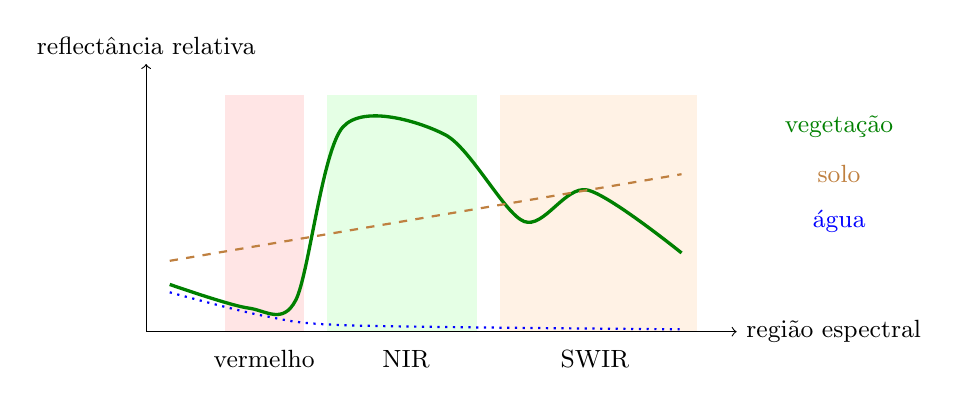
\begin{tikzpicture}[x=1cm,y=1cm,font=\small]
\fill[red!10] (1,0) rectangle (2,3);
\fill[green!10] (2.3,0) rectangle (4.2,3);
\fill[orange!10] (4.5,0) rectangle (7,3);
\draw[->] (0,0)--(7.5,0) node[right]{região espectral};
\draw[->] (0,0)--(0,3.4) node[above]{reflectância relativa};
\draw[very thick,green!50!black] plot[smooth] coordinates {(0.3,0.6)(1.3,0.3)(1.9,0.4)(2.5,2.6)(3.8,2.5)(4.8,1.4)(5.6,1.8)(6.8,1)};
\draw[thick,brown,dashed] (0.3,0.9)--(6.8,2);
\draw[thick,blue,dotted] plot[smooth] coordinates {(0.3,0.5)(1.5,0.2)(2.6,0.08)(6.8,0.03)};
\node at (1.5,-0.35){vermelho}; \node at (3.3,-0.35){NIR}; \node at (5.7,-0.35){SWIR};
\node[green!50!black] at (8.8,2.6){vegetação};
\node[brown] at (8.8,2){solo}; \node[blue] at (8.8,1.4){água};
\end{tikzpicture}
\caption{Comportamento espectral esquemático. Curvas qualitativas sem escala numérica, não medições. Fonte: elaborado pelo autor, síntese conceitual de \citet{WEISS2020}.}
\label{fig:espectro}
\end{figure*}
\begin{figure*}[htbp]
\centering\small
\begin{tabular}{lllll}
\hline Banda & Região & Centro S2A / S2B (nm) & Resolução & Índice no sistema\\ \hline
B4 & Vermelho & 664,5 / 665 & 10 m & NDVI\\
B8 & NIR amplo & 835,1 / 833 & 10 m & NDVI, NDWI\\
B8A & NIR estreito & 864,8 / 864 & 20 m & NDMI\\
B11 & SWIR & 1613,7 / 1610,4 & 20 m & NDWI, NDMI\\ \hline
\end{tabular}

\begin{tikzpicture}[x=0.009cm,y=0.6cm,font=\small]
\draw[->] (600,0)--(1730,0) node[right]{nm};
\foreach \x in {665,835,865,1614}{\draw[thick] (\x,0)--(\x,1);}
\node at (665,1.5){B4}; \node at (805,1.5){B8};
\node at (895,2){B8A}; \node at (1614,1.5){B11};
\end{tikzpicture}
\caption{Bandas dos índices. Centros espectrais por instrumento e resoluções nativas conforme o catálogo harmonizado \citep{GOOGLE_S2_SR}. Fonte: elaborado pelo autor.}
\label{fig:bandas}
\end{figure*}
\begin{figure*}[htbp]
\centering
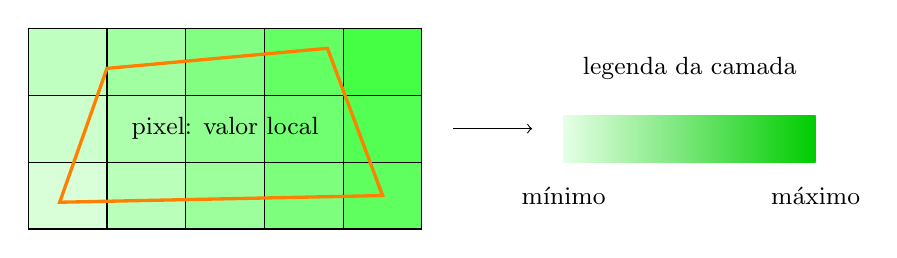
\begin{tikzpicture}[x=1cm,y=0.85cm,font=\small]
\foreach \x in {0,...,4}{\foreach \y in {0,...,2}{
\pgfmathtruncatemacro{\shade}{15+12*\x+5*\y}
\fill[green!\shade] (\x,\y) rectangle +(1,1);}}
\draw[step=1] (0,0) grid (5,3);
\draw[very thick,orange] (0.4,0.4)--(4.5,0.5)--(3.8,2.7)--(1,2.4)--cycle;
\node at (2.5,1.5){pixel: valor local};
\draw[->] (5.4,1.5)--(6.4,1.5);
\shade[left color=green!10,right color=green!80!black] (6.8,1) rectangle (10,1.7);
\node at (6.8,0.5){mínimo}; \node at (10,0.5){máximo};
\node at (8.4,2.4){legenda da camada};
\end{tikzpicture}
\caption{Polígono vetorial, células raster e gradiente em esquema sem dados reais. A geometria e as máscaras determinam o suporte válido. Fonte: elaborado pelo autor.}
\label{fig:raster-vetor}
\end{figure*}
\begin{figure*}[htbp]
\centering\small
\begin{tabular}{lcccl}
\hline & Pixel A & Pixel B & Média espacial & Operação\\ \hline
Aquisição 1 & 0,1 & 0,9 & 0,5 & média dos pixels\\
Aquisição 2 & 0,2 & 0,8 & 0,5 & média dos pixels\\
Aquisição 3 & 0,9 & 0,7 & 0,8 & média dos pixels\\ \hline
Mediana por pixel & 0,2 & 0,8 & 0,5 & média da composição\\ \hline
\end{tabular}
\caption{Ilustração matemática: a média das médias por aquisição é 0,6, enquanto a média da composição mediana é 0,5. Pesos iguais, sem máscaras; não é resultado experimental. Fonte: elaborado pelo autor.}
\label{fig:composicao}
\end{figure*}
\begin{figure*}[htbp]
\centering
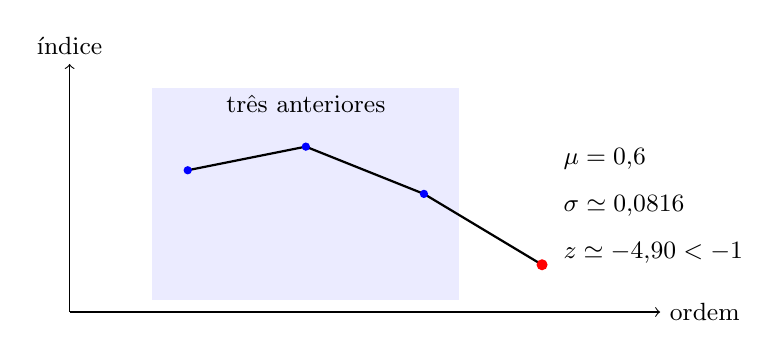
\begin{tikzpicture}[x=1.5cm,y=3cm,font=\small]
\fill[blue!8] (0.7,0.05) rectangle (3.3,0.95);
\draw[->] (0,0)--(5,0) node[right]{ordem};
\draw[->] (0,0)--(0,1.05) node[above]{índice};
\draw[thick] (1,0.6)--(2,0.7)--(3,0.5)--(4,0.2);
\foreach \x/\y in {1/0.6,2/0.7,3/0.5}{\fill[blue] (\x,\y) circle (1.5pt);}
\fill[red] (4,0.2) circle (2pt);
\node at (2,0.88){três anteriores};
\node[anchor=west] at (4.1,0.65){$\mu=0{,}6$};
\node[anchor=west] at (4.1,0.45){$\sigma\simeq0{,}0816$};
\node[anchor=west] at (4.1,0.25){$z\simeq-4{,}90<-1$};
\end{tikzpicture}
\caption{Janela e sinalização em sequência didática. Valores criados para ilustrar a regra, não observações agrícolas ou medida de eficácia. Fonte: elaborado pelo autor.}
\label{fig:janela}
\end{figure*}


\section{Trabalhos relacionados}\label{sec:relacionados-final}

O estudo de \citet{SLAIFFER2023} e sua publicação posterior \citep{SLAIFFER2025} investigam índices e produtividade da soja em áreas irrigadas e de sequeiro. Na publicação, mapas de produtividade da colhedora são relacionados a índices do Crop Monitoring por análises estatísticas e espaciais. Essa comparação evidencia uma diferença de objeto: enquanto o estudo investiga a relação entre indicadores e produtividade medida, este trabalho constrói o fluxo computacional que disponibiliza indicadores para exploração.

\citet{IZQUIERDO2026} integram sensores de campo, Sentinel-1, Sentinel-2 e dados agroclimáticos para modelar umidade em pomares de citros, com avaliação em anos independentes. A combinação de referência de campo e modelagem física e supervisionada permite avaliar estimativas de umidade. A plataforma aqui desenvolvida atua em outra etapa: organiza consulta, visualização e exportação de índices, sem treinamento de um estimador.

As revisões de \citet{WEISS2020} e \citet{PATRICIO2018} situam essas aplicações em um conjunto mais amplo de sensores e técnicas computacionais. Para este artefato, a questão central não é selecionar um modelo preditivo, mas coordenar representações, serviços e saídas de maneira verificável.

No monitoramento operacional, \citet{MERONI2019} examinam produtos MODIS utilizados pelo ASAP e pela autoridade de gestão de secas do Quênia. Seu tratamento de histórico sazonal, consolidação e erros mostra a importância da referência temporal para interpretar alertas. Em contraste, a regra deste sistema é exploratória e local à série; sua avaliação computacional não constitui avaliação de desempenho de um sistema de alerta agronômico.

No nível de infraestrutura, o Earth Engine oferece processamento programável, não substituindo a interface e os contratos desenvolvidos neste projeto \citep{GORELICK2017}. EOSDA Crop Monitoring e OneSoil são produtos finais. O guia oficial da EOSDA documenta desenho e importação de áreas, índices, gráficos, clima, leitura de valores por posição e downloads. Também diferencia recursos conforme plano e complementos \citep{EOSDA_GUIDE}. A página oficial da OneSoil documenta áreas, monitoramento espectral, comparação entre safras, clima e exportação de limites e mapas, distinguindo Mobile, Pro e assinaturas \citep{ONESOIL_PLATFORM_DETAIL}.

A \cref{tab:plataformas} apresenta uma comparação documental de funcionalidades, com fontes consultadas em novembro de 2026. EOSDA também oferece leitura por posição; a contribuição do artefato está na implementação documentada desse recurso e de seus contratos, não em sua exclusividade. A comparação não mede desempenho ou retorno financeiro.

\begin{table*}[htbp]
\centering\small
\caption{Comparação documental por finalidade e funcionalidades. As fontes oficiais dos produtos são \citet{EOSDA_GUIDE} e \citet{ONESOIL_PLATFORM_DETAIL}; Earth Engine é infraestrutura programável, não produto final equivalente. Recursos comerciais dependem de plano e modalidade.}
\label{tab:plataformas}
\setlength{\tabcolsep}{3pt}
\begin{tabular}{p{0.18\textwidth}p{0.18\textwidth}p{0.18\textwidth}p{0.18\textwidth}p{0.18\textwidth}}
\hline Critério & EOSDA & OneSoil & Earth Engine & Sistema\\ \hline
Natureza & Produto final & Produto final & Infraestrutura & Artefato acadêmico\\
Áreas & Desenho e importação & Desenho, seleção e upload & Geometrias por API & Desenho, nomes e GeoJSON\\
Exploração & Índices e gráficos por data & Monitoramento e comparação entre safras & Coleções e redutores & Composição e série por aquisição\\
Clima & Histórico e previsão & Clima e chuva & Integração por programação & Consulta diária NASA POWER\\
Saídas & Downloads documentados & Limites e mapas para máquinas & Exportação por programação & PDF, XLSX, CSV e GeoJSON\\
Acesso & Planos e complementos & Mobile/Pro e assinaturas & Projeto, elegibilidade e cotas & Web; cotas de serviços externos\\ \hline
\end{tabular}
\end{table*}

A distinção central é de finalidade: os produtos comerciais incluem gestão e recursos contratados; o Earth Engine oferece infraestrutura programável; e o artefato concentra um fluxo de seleção, processamento e exportação cuja implementação e verificação podem ser examinadas. Esse posicionamento permite discutir decisões de engenharia sem estabelecer superioridade funcional ou agronômica.
